%\addcontentsline{toc}{part}{Methods}
\part*{Methods}
In the present part, the hardware and software used in the project are explained, as well as the new software developed. 
The first chapter presents the different libraries and technologies that aided in the development of the thesis. 
In the second chapter, the code that has been developed in the project is explained.
Finally, the third chapter covers the hardware that is utilized.


%\addcontentsline{toc}{chapter}{Libraries and technologies}
\chapter{Libraries and technologies}
%%%%%%% explain why those technologies are being used !!!!
% technologies being used: 
%section or whatever

OpenCV\cite{opencv} (Open Source Computer Vision) is a library that implements real-time computer vision algorithms. 

It is cross-platform and it is released under a BSD\cite{BSD} license.

\begin{figure}[h]
	\begin{center}
    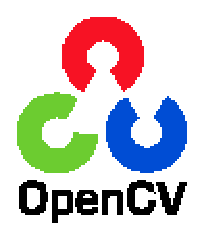
\includegraphics[scale=1]{img/opencv/logo.eps}
	\caption[OpenCV Logo]{OpenCV Logo}
	\end{center}
\end{figure}

\input{methods/pcl}
"The Robot Operating System (ROS) is a set of software libraries and tools that help you build robot applications. From drivers to state-of-the-art algorithms, and with powerful developer tools, ROS has what you need for your next robotics project. And it's all open source."\cite{ros}

\begin{figure}[h]
	\begin{center}
    
\includegraphics[scale=0.3]{img/ros/groovy.eps}
	\caption[ROS Groovy Logo]{ROS Groovy Logo}
	\end{center}
\end{figure}
 % here include all the packages that will be used in the code
%doxygen?? 

%\addcontentsline{toc}{chapter}{The Code}
\chapter{The Code}
  % diagrams & previous explanation of the code
  % nodes
  % communication between nodes
  % 
  
%%%%%%%%%% explain the reasons of chosing each library and method etc. !!!

%\addcontentsline{toc}{chapter}{Hardware}
\chapter{Hardware}
The hardware needed for the software of this project to work is an RGB-D sensor compatible with the openni\_launch ROS package previously mentioned, and a computer running a Linux distro. 
The sensor being used for the experiments presented in the following chapter is the Kinect of the Xbox 360. The reason of chosing this specific sensor is that it is cheaper than the other
and also more accesible. The drawback with respect to other sensors such as the Asus Xtion PRO LIVE\cite{xtion} is that it needs a separate power plug to work, and also its size is bigger. 
\\

The characteristics of the Kinect used are the following: 
%%%% complete with the characteristics that are now in the state of the art section --> they do not belong there!!



